\documentclass[a4paper, 10pt]{article}
\usepackage{amsmath}
\usepackage{fancyhdr}
\usepackage{float}
\usepackage[a4paper, left=1in, right=1in, top=1in, bottom=1in]{geometry} % Adjust margins
\usepackage{graphicx}
\usepackage{listings}
\usepackage{matlab-prettifier}

\pagestyle{fancy}

\title{ECE 340 Lab 1}
\author{Omar Mahmoud\\1753607\\Section D21}
\date{9/25/2024}

\lhead{Omar Mahmoud}
\rhead{ECE 340 Lab 1}
\headheight 15pt

\begin{document}

%% Cover Page
\thispagestyle{empty}
\vfill
\maketitle
\vfill

\newpage

%% (Q1) Signal Generation and Plotting
\section{Signal Generation and Plotting}

Consider the following discrete functions:
\begin{equation}
  x_1[k] = -5.1\sin(0.1\pi k-3\pi/4)\ -10\leq k\leq 10
\end{equation}
\begin{equation}
  x_2[k] = -(0.9)^ke^{(j\pi k/10)}\ 0\leq k\leq 100
\end{equation}

% Plotting x_1[k]
\noindent To start, $x_1[k]$ can be plotted on MATLAB through the following script:
\begin{lstlisting}[style=Matlab-editor, basicstyle=\small\ttfamily]
  subplot(2, 2, [1 2]);
  %% Define x_1
  k = -10:40;
  x1 = -5.1*sin(0.1*pi.*k - 3*pi/4) + 1.1*cos(0.4*pi.*k);
  %% Plot x_1
  stem(k, x1, 'LineWidth', 1, 'Color', 'b');
  title("Plot of x1[k].");
  xlabel("k");
  ylabel("x1[k]");
\end{lstlisting}
\begin{figure}[H]
  \centering
  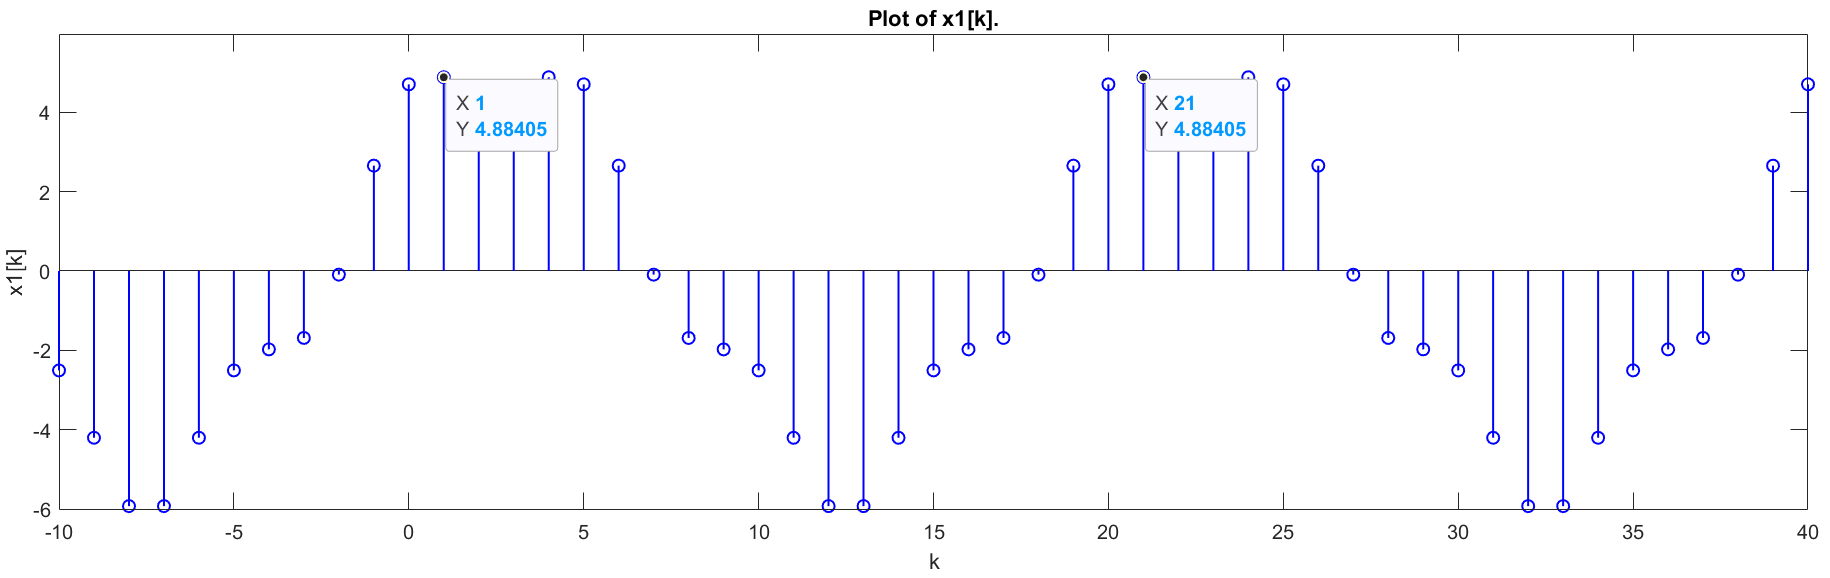
\includegraphics[width=15cm]{images/x1_plot.png}
  \caption{Plot of $x_1[k]$ with two points labeled to find the period.}
\end{figure}
By examining the graph, it is clear that $x_1[k]$ is a periodic sequence. To find the period, subtract 
the $X$ of the two selected points:
\begin{center}
  $T_{x_1} = X_2-X_1 = 21-1 = 20$ 
\end{center}

% Plotting x_2[k]
\noindent When plotting $x_2$ an imaginary and the real component will be produced. These can be plotted seperately 
through the following script:
\begin{lstlisting}[style=Matlab-editor, basicstyle=\small\ttfamily]
  %% Define x_2
  k = 0:100;
  x2 = (-0.9).^k .* exp(1).^(1j*pi.*k./10);
  %% Plot the real component of the x_2
  subplot(2, 2, 3);
  stem(k, real(x2),'LineWidth', 1, 'Color', 'r');
  title("Real Plot of x2[k].");
  xlabel("k");
  ylabel("Re(x2[k])");
  %% Plot the img component of x_2
  subplot(2, 2, 4);
  stem(k, imag(x2),'LineWidth', 1, 'Color', 'r');
  title("Imaginary Plot of x2[k].");
  xlabel("k");
  ylabel("Im(x2[k])");
\end{lstlisting}
\begin{figure}[H]
  \centering
  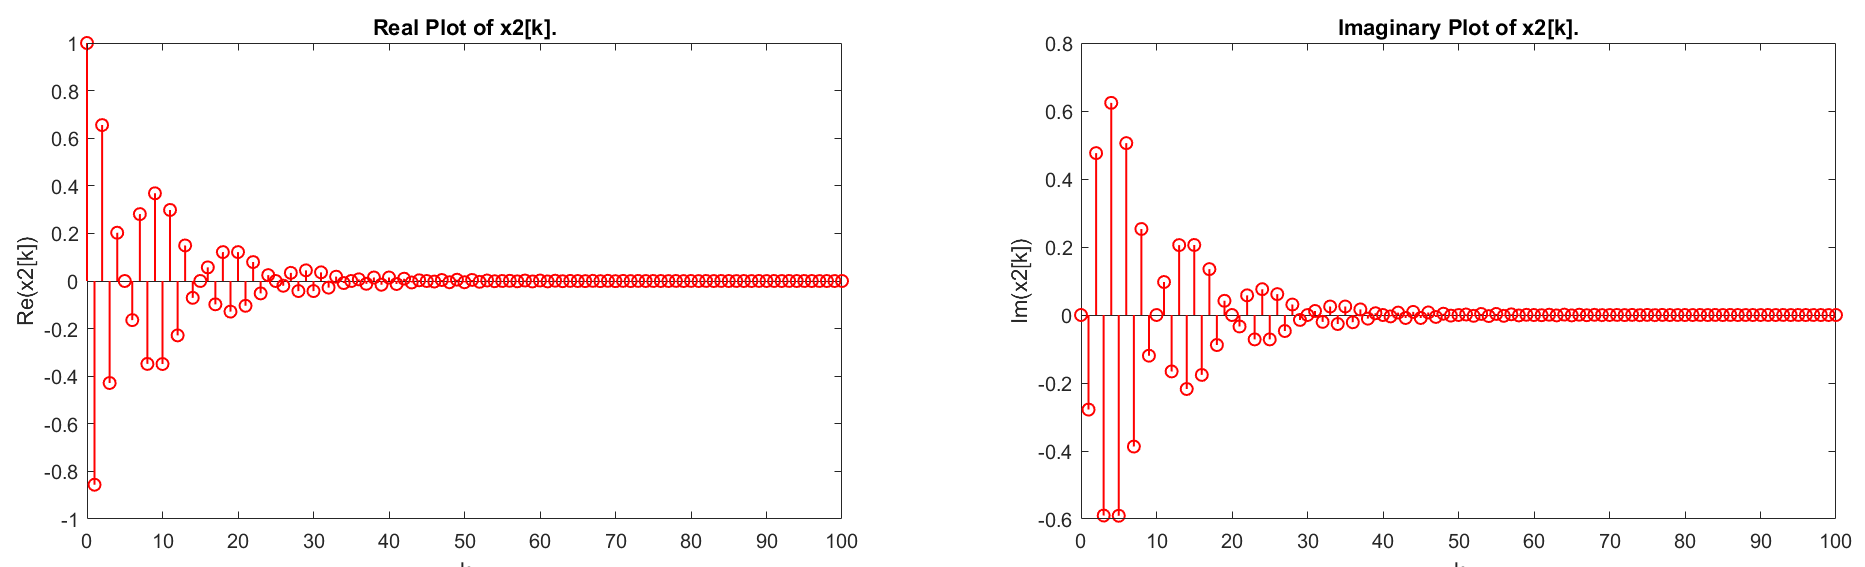
\includegraphics[width=15cm]{images/x2_plot.png}
  \caption{Plots of $Re(x_2[k])$ and $Im(x_2[k])$.}
\end{figure}
It is clear from the plots that $x_2[k]$ is not periodic, therefore it is not necessary to find a period.

\hfill

%% Finding the energy of x_1 and x_2
\noindent To find the total energy of the discrete-time signals $x_1[k]$ and $x_2[k]$ the following equation is used:
\begin{equation}
  E_x = \sum\limits_{n=-N}^{N} |x[n]|^2
\end{equation}
where $E_x$ represents the total energy of the signal over $[-N, N]$. The energy can be computed using the MATLAB script provided below:
\begin{lstlisting}[style=Matlab-editor, basicstyle=\small\ttfamily]
  %% Get energy of x_1
  fprintf('E_x1 = %.4f\n', sum(abs(x1).^2));
  %% Get energy of x_2
  fprintf('E_x2 = %.4f\n', sum(abs(x2).^2));
\end{lstlisting}
The output of the script is as follows:
\begin{lstlisting}[basicstyle=\small\ttfamily]
  E_x1 = 698.5335
  E_x2 = 5.2632
\end{lstlisting}

%% (Q2) Digital Audio
\section{Digital Audio}

MATLAB provides features that facilitate the reading and writing of audio signals from and to .wav files.
The following script reads the audio file \textbf{baila.wav}, and stores its audio signal into the matrix,
$x_3$ along with its sampling rate in $F_s$. In this context, the rows of $x_3$ represents the samples, while
the columns represent the channels of the audio signal:
\begin{lstlisting}[style=Matlab-editor, basicstyle=\small\ttfamily]
  %% Read the audio file baila.wav
  [x3, Fs] = audioread('baila.wav');
  [num_samples, num_channels] = size(x3);
  disp(['Number of samples: ', num2str(num_samples)]);
  disp(['Number of channels: ', num2str(num_channels)]);
\end{lstlisting}
The output of the script is as follows:
\begin{lstlisting}[basicstyle=\small\ttfamily]
  Number of samples: 1000000
  Number of channels: 1
\end{lstlisting}
From the output, it is evident \textbf{baila.wav} contains a mono-channel signal with 1,000,000 samples.
To analyze this signal, the next step involves creating an apporpriate time vector and plotting the mono signal
against it using the following script:
\begin{lstlisting}[style=Matlab-editor, basicstyle=\small\ttfamily]
  %% Create time vector
  t = (0:num_samples-1) / Fs;
  %% Plot the audio signal against it
  figure(1);
  plot(t, x3);
  ylabel('Amplitude');
  xlabel('Time (seconds)');
  title('Audio Signal over Time');
\end{lstlisting}
\begin{figure}[H]
  \centering
  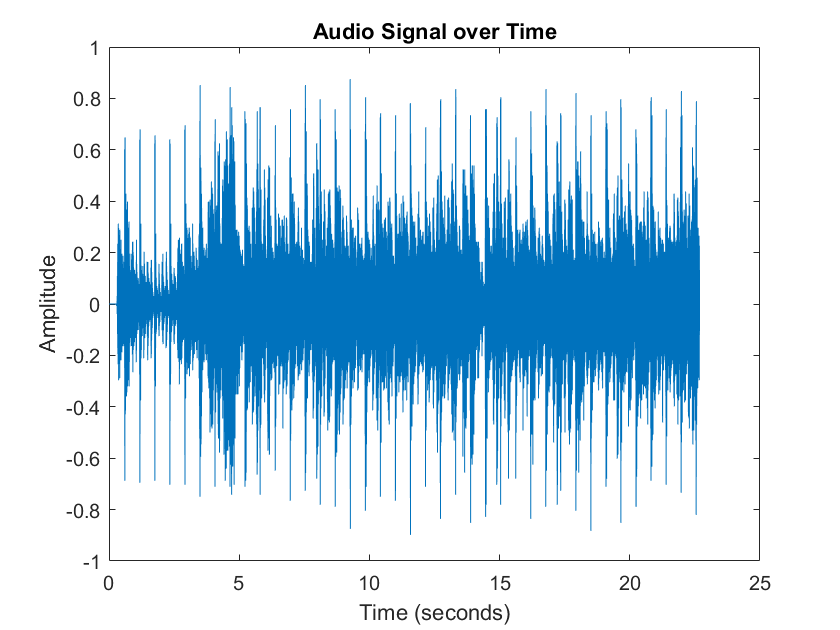
\includegraphics[width=8cm]{images/x3_plot.png}
  \caption{Plot of the mono audio signal $x_3$ extracted from \textbf{baila.wav}.}
\end{figure}
To assess the total energy of $x_3$ the same method as Section 1 is employed:
\begin{lstlisting}[style=Matlab-editor, basicstyle=\small\ttfamily]
  %% Get total energy
  fprintf('E_x3 = %.4f\n', sum(abs(x3).^2));
\end{lstlisting}
The value generated by the script is as follows:
\begin{lstlisting}[basicstyle=\small\ttfamily]
  E_x3 = 20422.7731
\end{lstlisting}

\hfill

\noindent To showcase MATLAB's audio writing features, the following script samples the first half of the matrix 
$x_3$ and creates a new matrix $x_{3s}$. This matrix is then used to play half of the \textbf{baila.wav} file 
using MATLAB's \textit{sound} function and generates a new \textbf{baila\_half.wav} file using the
\textit{audiowrite} function:
\begin{lstlisting}[style=Matlab-editor, basicstyle=\small\ttfamily]
  %% Get x3s, play it, and create baila_half.wav
  x3s = x3(1:floor(num_samples/2), :);
  sound(x3s, Fs);
  audiowrite('baila_half.wav', x3s, Fs);  
\end{lstlisting}

%% (Q3) Digital Image
\section{Digital Image}
MATLAB provides features that facilitate the reading and writing from and to JPEG image files.
The following script reads the JPEG file \textbf{vase.jpg}, and stores its value into the matrix \textit{vase}:
\begin{lstlisting}[style=Matlab-editor, basicstyle=\small\ttfamily]
  %% read the jpg file and get metrics
  vase = imread('vase.jpg');
  [rows, cols] = size(vase);
  max_pixel = max(vase(:));
  
  disp(['Number of rows: ', num2str(rows)]);
  disp(['Number of cols: ',  num2str(cols)]);
  disp(['Max pixel value: ',  num2str(max_pixel)]);
\end{lstlisting}
The output of script returns the number of rows, columns, and the maximum pixel value of the image:
\begin{lstlisting}[basicstyle=\small\ttfamily]
  Number of rows: 512
  Number of cols: 1083
  Max pixel value: 255
\end{lstlisting}
MATLAB also facilitates the creation of new JPEG files. Below \textit{imwrite} is utilized to create a new
image \textbf{vase\_bright.jpg}, by adding 30 to all the pixel values of the original image.
This results in a visually brighter version of the original \textbf{vase.jpg}:
\begin{lstlisting}[style=Matlab-editor, basicstyle=\small\ttfamily]
  %% create the new bright jpg
  vase_bright = vase + 30;
  imwrite(vase_bright, 'vase_bright.jpg', 'jpg', 'Quality', 100);
\end{lstlisting}
\begin{figure}[H]
  \centering
  
\includegraphics[width=5cm]{images/vase.jpg}
  
\includegraphics[width=5cm]{images/vase_bright.jpg}
  \caption{Comparison of the original \textbf{vase.jpg} (right) and the brightened \textbf{vase\_bright.jpg} (left).}
\end{figure}

%% (Q4) System Response
\section{System Response}
The schematic of a discrete-time signal is given below:
\begin{figure}[H]
  \centering
  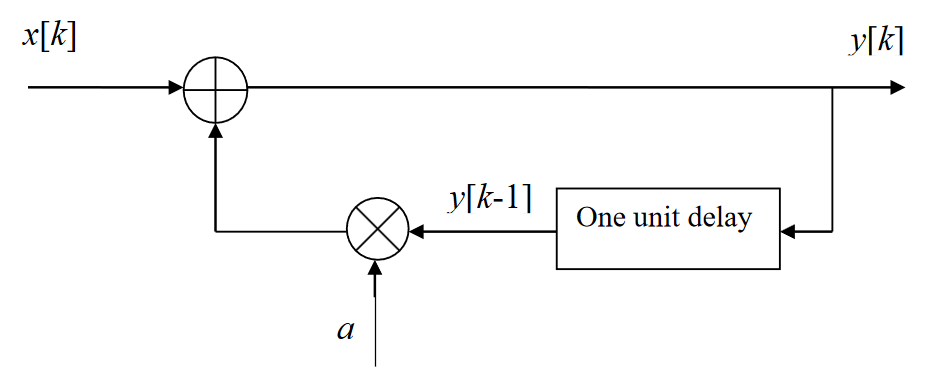
\includegraphics[width=10cm]{images/system_schem.png}
  \caption{Schematic of the discrete-time signal for this section.}
\end{figure}
\noindent The relationship between $x[k]$ and $y[k]$ can be expressed as:
\begin{equation}
  y[k] = x[k]+ay[k-1]
\end{equation}
%%Manually get y[k]
Assuming that x[k] is a unit-step function and $y[k] = 0$ for $k<0$,
the $y[k]$ of the system for $0 \leq k < 5$ for (i) $a=0.5$ and (ii) $a=5$ can
be computed manually:

\hfill

\noindent i) when $a=0.5$:
\begin{center}
  $y[0]=x[0]+0.5y[-1]=(1)+0.5(0)=1$\\
  $y[1]=x[1]+0.5y[0]=(1)+0.5(1)=1.5$\\
  $y[2]=x[2]+0.5y[1]=(1)+0.5(1.5)=1.75$\\
  $y[3]=x[3]+0.5y[2]=(1)+0.5(1.75)=1.875$\\
  $y[4]=x[4]+0.5y[3]=(1)+0.5(1.875)=1.9375$\\
\end{center}
ii) when $a=5$
\begin{center}
  $y[0]=x[0]+5y[-1]=(1)+5(0)=1$\\
  $y[1]=x[1]+5y[0]=(1)+5(1)=6$\\
  $y[2]=x[2]+5y[1]=(1)+5(6)=31$\\
  $y[3]=x[3]+5y[2]=(1)+5(31)=156$\\
  $y[4]=x[4]+5y[3]=(1)+5(156)=781$\\
\end{center}

\hfill

\noindent To get y[k] for $0 \leq k < 50$, it is more time efficient to use MATLAB.
Below is the function \textit{sysresp}, which calculates and plots the apporpriate
$y[k]$ for a given input $x[k]$ and system parameter $a$:
\begin{lstlisting}[style=Matlab-editor, basicstyle=\small\ttfamily]
  function y=sysresp(x, a)
  %
  % Computes the output in response to an arbitrary input x[n], n=0, ...N-1.
  % Assume that the system has 0 initial conditions.
  % Input:
  %   x: the input signal,
  %   a: the system parameter
  % Output:
  %   y: the output signal

  N = length(x); % length of the vector
  y = zeros(1, N);

  for k = 1:N+1
    if k == 1
      y(k) = 1;
    else
      y(k) = 1 + a * y(k-1);
    end
  end

  figure(1)
  stem(1:N+1, y,'LineWidth', 1, 'Color', 'b');
  title(['Plot of y[k] when a = ', num2str(a), '.']);
  xlabel('k');
  ylabel('y[k]');
  return
\end{lstlisting}
When we use this function with the system parameters $a=0.5$ and $a=5$,
we get the following plots:
\begin{figure}[H]
  \centering
  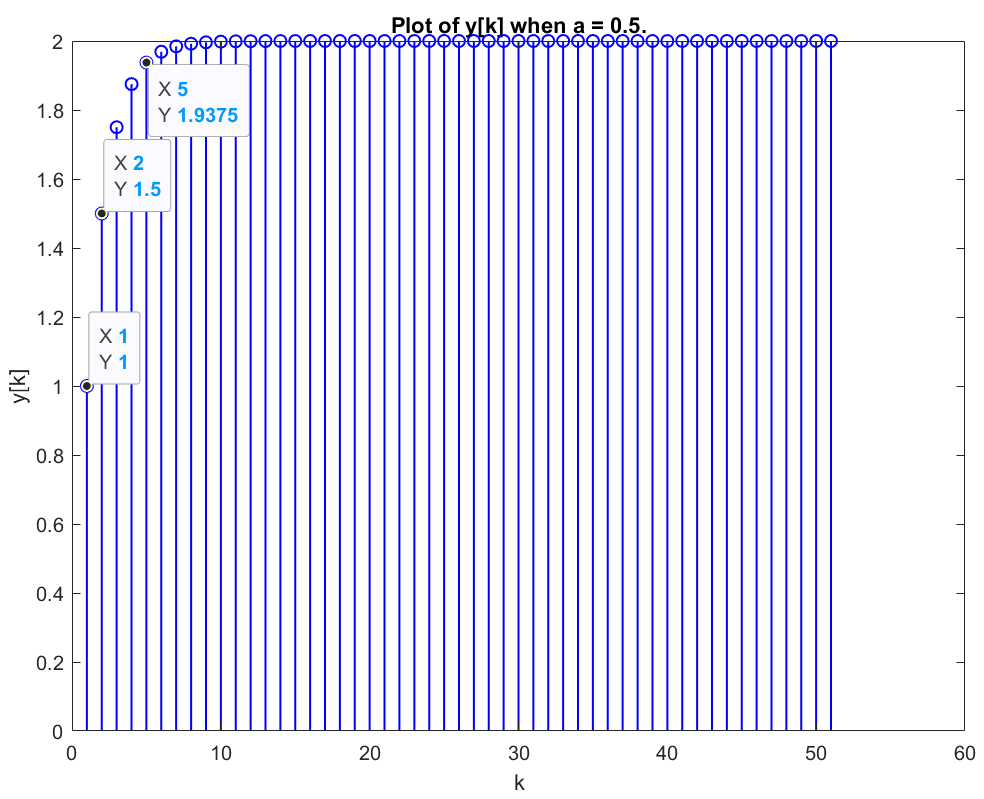
\includegraphics[width=10cm]{images/yk_graph_1.png}
  \caption{Plot of $y[k]$ when $a=0.5$}
\end{figure}
\begin{figure}[H]
  \centering
  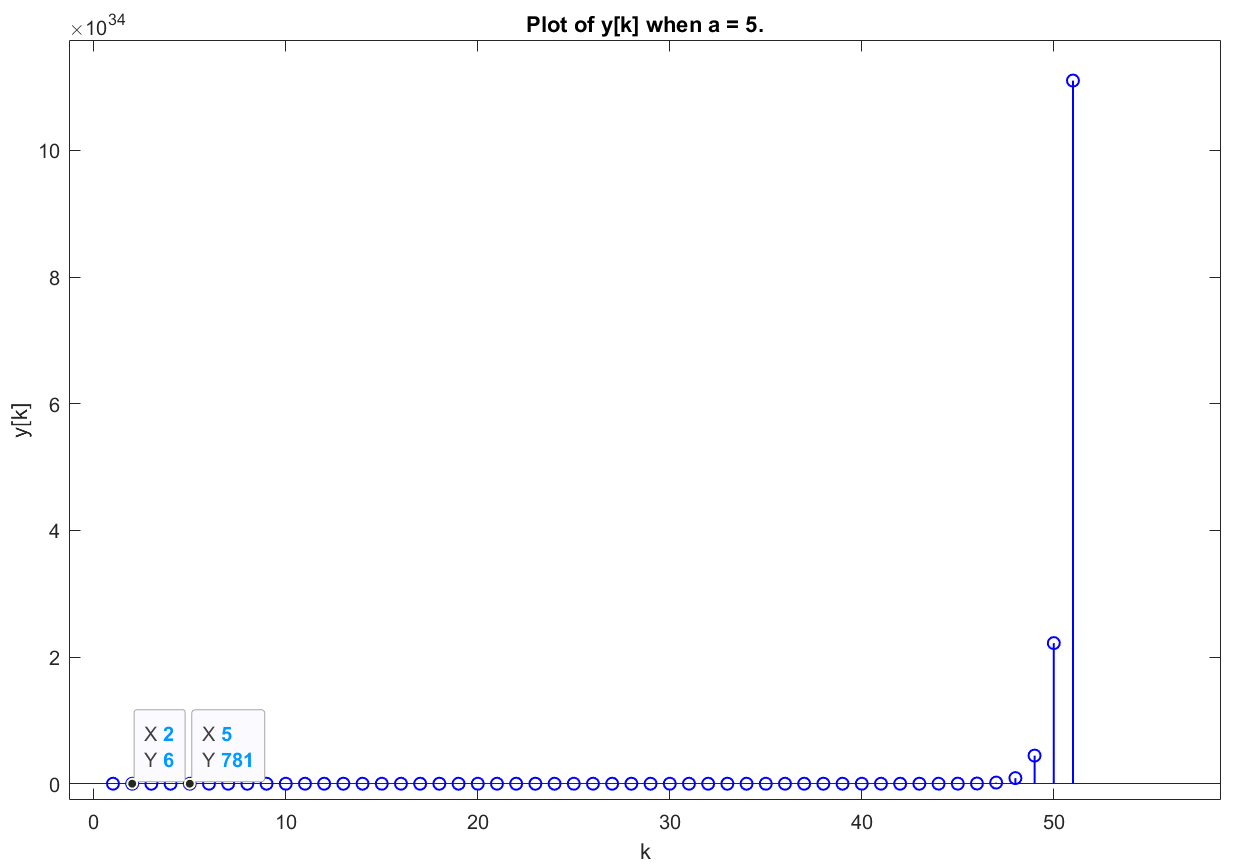
\includegraphics[width=10cm]{images/yk_graph_2.png}
  \caption{Plot of $y[k]$ when $a=5$}
\end{figure}
\noindent Upon examining the graphs, it is evident that the results from \textit{sysresp} match the 
initial hand calculations. It is also evident that $y[k]$ is bounded showing a BIBO stable
signal for $a=0.5$, but is not bounded $a=5$ showing a BIBO unstable signal.

\hfill

\noindent Another $a$ value that would allow for a BIBO stable signal is $0.2$. This can be confirmed using
the \textit{sysresp} function:
\begin{lstlisting}[style=Matlab-editor, basicstyle=\small\ttfamily]
  x = ones(1, 50);
  sysresp(x, 0.2);
\end{lstlisting}
\begin{figure}[H]
  \centering
  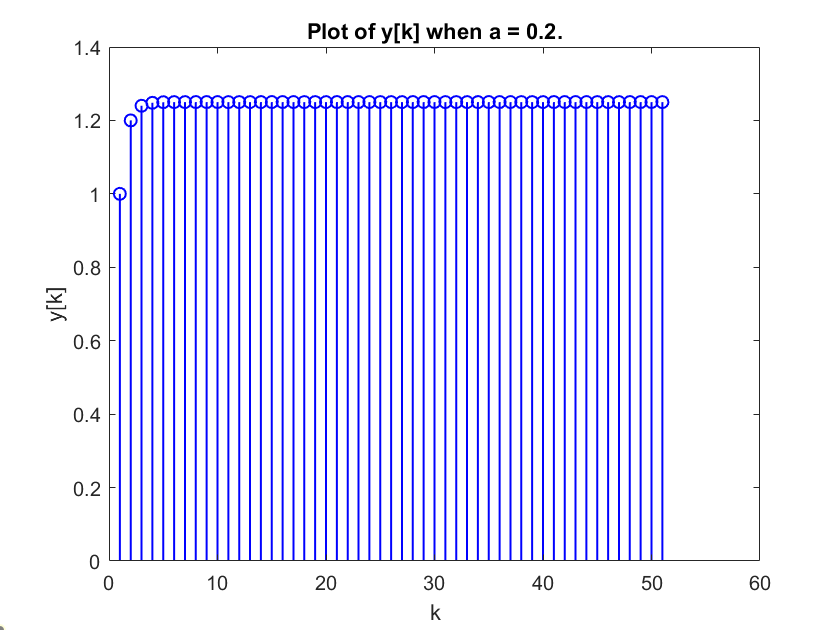
\includegraphics[width=10cm]{images/yk_graph_3.png}
  \caption{Plot of $y[k]$ when $a=0.2$}
\end{figure}
Upon examining the graph, it is clear that $y[k]$ is bounded showing a BIBO stable signal for $a=0.2$.
\end{document}